\begin{figure}[h]
  \vspace{4mm}
  \centering
  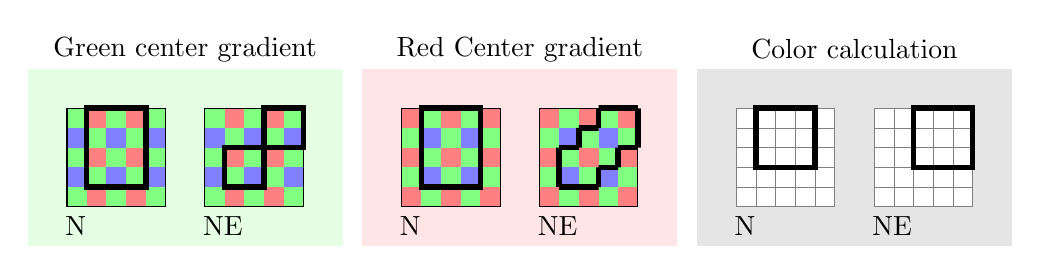
\begin{tikzpicture}
    \node[] at (1.5,2) {Green center gradient};
    \fill[fill=green!10] (-0.5,-0.5) rectangle (3.5,1.75);
    \node[] at (5.75,2) {Red Center gradient};
    \fill[fill=red!10] (3.75,-0.5) rectangle (7.75,1.75);
    \node[] at (10,2) {Color calculation};
    \fill[fill=black!10] (8,-0.5) rectangle (12,1.75);
    \begin{scope}[shift={(0,0)}, local bounding box=sensorin]
      \filldraw[fill=green!50]   (0,0)     rectangle (1.25,1.25);

      \fill[fill=blue!50] (.0,.25) rectangle (.25,.5);
      \fill[fill=blue!50] (.0,.75) rectangle (.25,1);
      \fill[fill=blue!50] (.5,.25) rectangle (.75,.5);
      \fill[fill=blue!50] (.5,.75) rectangle (.75,1);
      \fill[fill=blue!50] (1,.25) rectangle (1.25,.5);
      \fill[fill=blue!50] (1,.75) rectangle (1.25,1);

      \fill[fill=red!50]  (.25,0)     rectangle (.5,.25);
      \fill[fill=red!50]  (.25,.5)    rectangle (.5,.75);
      \fill[fill=red!50]  (.25,1)     rectangle (.5,1.25);
      \fill[fill=red!50]  (.75,0)     rectangle (1,.25);
      \fill[fill=red!50]  (.75,.5)    rectangle (1,.75);
      \fill[fill=red!50]  (.75,1)     rectangle (1,1.25);

      \draw[line width=2pt] (.25, .25) rectangle (1, 1.25);
      \node[text width = 1.25] at (.0, -.25) {N};
      \draw[] (0,0)     rectangle (1.25,1.25);
    \end{scope}
    \begin{scope}[shift={(1.75,0)}, local bounding box=sensorin]
      \filldraw[fill=green!50]   (0,0)     rectangle (1.25,1.25);

      \fill[fill=blue!50] (.0,.25) rectangle (.25,.5);
      \fill[fill=blue!50] (.0,.75) rectangle (.25,1);
      \fill[fill=blue!50] (.5,.25) rectangle (.75,.5);
      \fill[fill=blue!50] (.5,.75) rectangle (.75,1);
      \fill[fill=blue!50] (1,.25) rectangle (1.25,.5);
      \fill[fill=blue!50] (1,.75) rectangle (1.25,1);

      \fill[fill=red!50]  (.25,0)     rectangle (.5,.25);
      \fill[fill=red!50]  (.25,.5)    rectangle (.5,.75);
      \fill[fill=red!50]  (.25,1)     rectangle (.5,1.25);
      \fill[fill=red!50]  (.75,0)     rectangle (1,.25);
      \fill[fill=red!50]  (.75,.5)    rectangle (1,.75);
      \fill[fill=red!50]  (.75,1)     rectangle (1,1.25);

      \draw[line width=2pt] (.25, .25) rectangle (.75, .75);
      \draw[line width=2pt] (.75, .75) rectangle (1.25, 1.25);
      \node[text width = 1.25] at (.0, -.25) {NE};
      \draw[] (0,0)     rectangle (1.25,1.25);
    \end{scope}

    \begin{scope}[shift={(4.25,0)}, local bounding box=sensorin]
      \filldraw[fill=green!50]   (0,0)     rectangle (1.25,1.25);
      \fill[fill=red!50]  (0,0)     rectangle (.25,.25);
      \fill[fill=red!50]  (.5,0)    rectangle (.75,.25);
      \fill[fill=red!50]  (.5,.5)   rectangle (.75,.75);
      \fill[fill=red!50]  (0,.5)    rectangle (.25,.75);

      \fill[fill=red!50]  (1,1)     rectangle (1.25,1.25);
      \fill[fill=red!50]  (.5,1)    rectangle (.75,1.25);
      \fill[fill=red!50]  (1,.5)    rectangle (1.25,.75);

      \fill[fill=red!50]  (0,1)     rectangle (.25,1.25);
      \fill[fill=red!50]  (1,0)     rectangle (1.25,.25);

      \fill[fill=blue!50] (.25,.25) rectangle (.5,.5);
      \fill[fill=blue!50] (.75,.25) rectangle (1,.5);
      \fill[fill=blue!50] (.25,.75) rectangle (.5,1);
      \fill[fill=blue!50] (.75,.75) rectangle (1,1);

      \draw[line width=2pt] (.25, .25) rectangle (1, 1.25);
      \node[text width = 1.25] at (.0, -.25) {N};
      \draw[] (0,0)     rectangle (1.25,1.25);
    \end{scope}
    \begin{scope}[shift={(6,0)}, local bounding box=sensorin]
      \filldraw[fill=green!50]   (0,0)     rectangle (1.25,1.25);
      \fill[fill=red!50]  (0,0)     rectangle (.25,.25);
      \fill[fill=red!50]  (.5,0)    rectangle (.75,.25);
      \fill[fill=red!50]  (.5,.5)   rectangle (.75,.75);
      \fill[fill=red!50]  (0,.5)    rectangle (.25,.75);

      \fill[fill=red!50]  (1,1)     rectangle (1.25,1.25);
      \fill[fill=red!50]  (.5,1)    rectangle (.75,1.25);
      \fill[fill=red!50]  (1,.5)    rectangle (1.25,.75);

      \fill[fill=red!50]  (0,1)     rectangle (.25,1.25);
      \fill[fill=red!50]  (1,0)     rectangle (1.25,.25);

      \fill[fill=blue!50] (.25,.25) rectangle (.5,.5);
      \fill[fill=blue!50] (.75,.25) rectangle (1,.5);
      \fill[fill=blue!50] (.25,.75) rectangle (.5,1);
      \fill[fill=blue!50] (.75,.75) rectangle (1,1);

      \draw[line width=2pt] (.25, .25) rectangle (.75, .25);
      \draw[line width=2pt] (.25, .25) rectangle (.25, .75);

      \draw[line width=2pt] (.75, .25) rectangle (.75, .5);
      \draw[line width=2pt] (.25, .75) rectangle (.5, .75);

      \draw[line width=2pt] (.75, .5) rectangle (1, .5);
      \draw[line width=2pt] (.5, .75) rectangle (.5, 1);

      \draw[line width=2pt] (1, .5) rectangle (1, .75);
      \draw[line width=2pt] (.5, 1) rectangle (.75, 1);

      \draw[line width=2pt] (1, .75) rectangle (1.25, .75);
      \draw[line width=2pt] (.75, 1) rectangle (.75, 1.25);

      \draw[line width=2pt] (1.25, .75) rectangle (1.25, 1.25);
      \draw[line width=2pt] (.75, 1.25) rectangle (1.25, 1.25);
      \node[text width = 1.25] at (.0, -.25) {NE};
      \draw[] (0,0)     rectangle (1.25,1.25);
    \end{scope}

    \begin{scope}[shift={(8.5,0)}, local bounding box=sensorin]
      \fill[white] (0,0) rectangle (1.25,1.25);
      \draw[black!50, step=.25,very thin] (0,0) grid (1.25,1.25);

      \draw[line width=2pt] (.25, .5) rectangle (1, 1.25);
      \node[text width = 1.25] at (.0, -.25) {N};
    \end{scope}

    \begin{scope}[shift={(10.25,0)}, local bounding box=sensorin]
      \fill[white] (0,0) rectangle (1.25,1.25);
      \draw[black!50, step=.25,very thin] (0,0) grid (1.25,1.25);

      \draw[line width=2pt] (.5, .5) rectangle (1.25, 1.25);
      \node[text width = 1.25] at (.0, -.25) {NE};
    \end{scope}

  \end{tikzpicture}
  \caption{VNG gradient and color calculation regions, only North and North East regions are included. Other regions can be constructed by rotating these regions by 90, 180, and 270 degrees.}
  \label{fig:vng}
  \vspace{4mm}
\end{figure}
